%%%%%%%%%%%%%%%%%%%%%%%%%%%%%%%%%%%%%%%%%
% Short Sectioned Assignment
% LaTeX Template
% Version 1.0 (5/5/12)
%
% This template has been downloaded from:
% http://www.LaTeXTemplates.com
%
% Original author:
% Frits Wenneker (http://www.howtotex.com)
%
% License:
% CC BY-NC-SA 3.0 (http://creativecommons.org/licenses/by-nc-sa/3.0/)
%
%%%%%%%%%%%%%%%%%%%%%%%%%%%%%%%%%%%%%%%%%

%----------------------------------------------------------------------------------------
%	PACKAGES AND OTHER DOCUMENT CONFIGURATIONS
%----------------------------------------------------------------------------------------

\documentclass[paper=a4, fontsize=11pt]{scrartcl} % A4 paper and 11pt font size

\usepackage[T1]{fontenc} % Use 8-bit encoding that has 256 glyphs
\usepackage{fourier} % Use the Adobe Utopia font for the document - comment this line to return to the LaTeX default
\usepackage[english]{babel} % English language/hyphenation
\usepackage{amsmath,amsfonts,amsthm} % Math packages
\usepackage{pgfplots, tikz}
\usetikzlibrary{intersections}
\usepackage[CJKbookmarks=true,
            colorlinks,linkcolor=black,anchorcolor=blue,citecolor=green]{hyperref}

\usepackage{lipsum} % Used for inserting dummy 'Lorem ipsum' text into the template

\usepackage{sectsty} % Allows customizing section commands
\allsectionsfont{\centering \normalfont\scshape} % Make all sections centered, the default font and small caps

\usepackage{fancyhdr} % Custom headers and footers
\pagestyle{fancyplain} % Makes all pages in the document conform to the custom headers and footers
\fancyhead{} % No page header - if you want one, create it in the same way as the footers below
\fancyfoot[L]{} % Empty left footer
\fancyfoot[C]{} % Empty center footer
\fancyfoot[R]{\thepage} % Page numbering for right footer
\renewcommand{\headrulewidth}{0pt} % Remove header underlines
\renewcommand{\footrulewidth}{0pt} % Remove footer underlines
\renewcommand\thesection{\roman{section}}

\setlength{\headheight}{13.6pt} % Customize the height of the header

\numberwithin{equation}{section} % Number equations within sections (i.e. 1.1, 1.2, 2.1, 2.2 instead of 1, 2, 3, 4)
\numberwithin{figure}{section} % Number figures within sections (i.e. 1.1, 1.2, 2.1, 2.2 instead of 1, 2, 3, 4)
\numberwithin{table}{section} % Number tables within sections (i.e. 1.1, 1.2, 2.1, 2.2 instead of 1, 2, 3, 4)

\setlength\parindent{0pt} % Removes all indentation from paragraphs - comment this line for an assignment with lots of text

%----------------------------------------------------------------------------------------
%	TITLE SECTION
%----------------------------------------------------------------------------------------

\newcommand{\horrule}[1]{\rule{\linewidth}{#1}} % Create horizontal rule command with 1 argument of height

\title{	
\normalfont \normalsize
\textsc{School of Software, Tsinghua University} \\ [25pt] % Your university, school and/or department name(s)
\horrule{0.5pt} \\[0.4cm] % Thin top horizontal rule
\huge Optimization Method\\ % The assignment title
\LARGE\textit{homework 1}
\horrule{2pt} \\[0.5cm] % Thick bottom horizontal rule
}

\author{Qingfu Wen \\ \normalsize 2015213495} % Your Info
\date{\normalsize\today} % Today's date or a custom date

\begin{document}

\maketitle % Print the title
\tableofcontents
\newpage
%----------------------------------------------------------------------------------------
%	PROBLEM 1
%----------------------------------------------------------------------------------------

\section{Problem 1}
Prove the following set $S$ is a convex set.
\begin{equation}  \nonumber
S = \{x|x=Ay, y\geq0\}
\end{equation}
$A$ is a $n*m$ matrix, $x\in \mathbb{R}^n$,$y\in \mathbb{R}^m$.\\
\emph{\textbf{Proof:}}\\
$\forall x^{(1)}, x^{(2)}\in S, \forall \lambda \in [0, 1]$, then $x^{(1)}=Ay_1, x^{(2)}=Ay_2, y_1,y_2\geq0$.
\begin{align*}          
& \lambda x^{(1)}+(1-\lambda)x^{(2)}\\         
=& \lambda Ay_1+(1-\lambda)Ay_2\\      
=& A[\lambda y_1+(1-\lambda)y_2]\\      
\end{align*}
because $y_1,y_2\geq0,\lambda\in[0,1]$, $\lambda y_1+(1-\lambda)y_2\geq0$. Then, $\lambda x^{(1)}+(1-\lambda)x^{(2)} \in S$.\\
So, $S$ is a convex set.
\section{Problem 2}
Suppose $S$ is a nonempty convex set of $E^n$. Prove for all integer $k \geq 2$, if $x^{(1)}$,$x^{(2)}$,$\cdots$,$x^{(k)} \in S$, then
\begin{equation} \nonumber
\sum_{i=1}^{k}\lambda_ix^{(i)}\in S
\end{equation}
among it, $\lambda_1+\lambda_2+\cdots+\lambda_k=1, \lambda_i \geq 0, i=1,\cdots,k$.\\
\emph{\textbf{Proof:}}
\begin{enumerate}
\item Using mathematical induction, when $k=2$, the above formula holds because of the definition of \textbf{convex set}.
\item Suppose when $k=n$, the formula holds. Then when $k=n+1$, we have
\begin{align*}
& \sum_{i=1}^{n+1} \lambda_ix^{(i)} \\
=& \sum_{i=1}^{n} \lambda_ix^{(i)}+\lambda_{n+1}x^{(n+1)}\\
=& \sum_{i=1}^{n} \lambda_i\big[\sum_{i=1}^{n}\frac{\lambda_i}{\sum_{i=1}^{n}\lambda_i}x^{(i)}\big]+\lambda_{n+1}x^{(n+1)}\\
\end{align*}
Among it, $\sum_{i=1}^{n+1} \lambda_i=1$, from the hypothesis, we know $\sum_{i=1}^{n}\frac{\lambda_i}{\sum_{i=1}^{n}\lambda_i}x^{(i)} \in S$. Moreover, because $\sum_{i=1}^{n} \lambda_+\lambda_{n+1}=1$, therefore $\sum_{i=1}^{n} \lambda_i\big[\sum_{i=1}^{n}\frac{\lambda_i}{\sum_{i=1}^{n}\lambda_i}x^{(i)}+\lambda_{n+1}x^{(n+1)}\big] \in S$.\\
So, when $k=n+1$, the formula holds.
\item Finally, for all $k$, $\sum_{i=1}^{k}\lambda_ix^{(i)}\in S$.
\end{enumerate}
\section{Problem 3}
Solve the following linear programming problem using graphical method.\\
(4)
\begin{flalign*}          \nonumber
\min\quad & -20x_1+10x_2\\  \nonumber
\mbox{s.t.}\quad            \nonumber
& x_1+x_2 \geq 10\\         \nonumber
& -10x_1+x_2 \leq 10\\      \nonumber
& -5x_1+5x_2 \leq 25\\      \nonumber
& x_1+4x_2 \geq 20\\        \nonumber
& x_1,x_2 \geq 0
\end{flalign*}

\emph{\textbf{Solution:}}\\
From the following graph, we can see that when $x_1=2.5, x_2=7.5$, $-20x_1+10x_2$ can reach the maximum value 25.\\
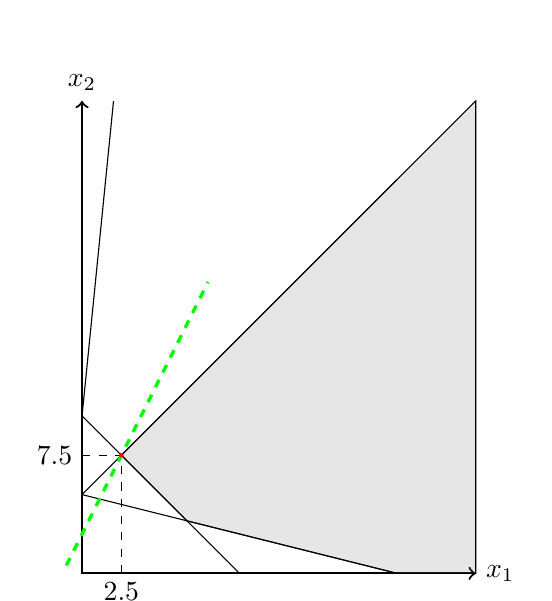
\begin{tikzpicture}[scale=0.2]
    % Draw axes
    \draw [<->,thick] (0,30) node (yaxis) [above] {$x_2$}
        |- (25,0) node (xaxis) [right] {$x_1$};
    % Draw lines
    
    \draw [-,samples=100,domain=0:10, name path = A] plot(\x,{10-\x});
    \draw [-,samples=100,domain=0:20, name path = B] plot(\x,{5+\x});
    \draw [-,samples=100,domain=0:20, name path = C] plot(\x,{5-0.25*\x});
    \draw [-,samples=100,domain=0:2, name path = D] plot(\x,{10+10*\x});
    \draw [-,samples=100,dashed, very thick, green, domain=-1:8] plot(\x,{2*\x+2.5});
    
    \draw [fill=gray,fill opacity=0.2] plot [smooth,samples=100,domain=2.5:6.6667](\x,{10-\x})-- plot [smooth,samples=100,domain=6.6667:20](\x,{5-0.25*\x}) -- (25, 0) -- plot [smooth,samples=100,domain=25:2.5] (\x,{5+\x});

    % Calculate the intersection of the lines a_1 -- a_2 and b_1 -- b_2
    % and store the coordinate in c.
    %\draw [fill=gray,fill opacity=0.2] A--B;

    \coordinate (c) at (2.5, 7.5);
    % Draw lines indicating intersection with y and x axis. Here we use
    % the perpendicular coordinate system
    \draw[dashed] (yaxis |- c) node[left] {$7.5$}
        -| (xaxis -| c) node[below] {$2.5$};
    % Draw a dot to indicate intersection point
    \fill[red] (c) circle (4pt);
\end{tikzpicture}

(5)
\begin{alignat}{2}          \nonumber
\min\quad & -3x_1-2x_2\\    \nonumber
\mbox{s.t.}\quad            \nonumber
& 3x_1+2x_2 \leq 6\\        \nonumber
& x_1-2x_2 \leq 1\\         \nonumber
& x_1+x_2 \geq 1\\          \nonumber
& -x_1+2x_2 \leq 1\\        \nonumber
& x_1,x_2 \geq 0
\end{alignat}

\emph{\textbf{Solution:}}\\
From the following graph, we can see that from ($\frac{5}{4}$,$\frac{9}{8}$) to ($\frac{7}{4}$,$\frac{3}{8}$), $-3x_1-2x_2$ reaches the minimum value -6, e.g. $x_1=\frac{7}{4},x_2=\frac{3}{8}$.\\
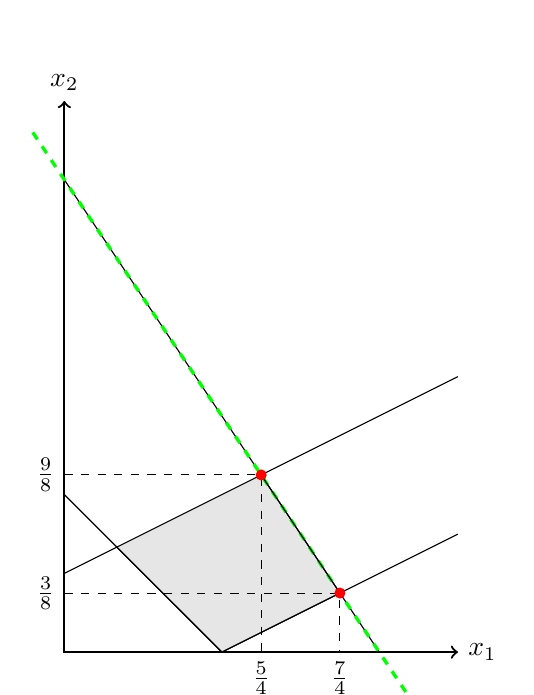
\begin{tikzpicture}[scale=2]
    % Draw axes
    \draw [<->,thick] (0,3.5) node (yaxis) [above] {$x_2$}
        |- (2.5,0) node (xaxis) [right] {$x_1$};
    % Draw lines
    \draw [-,samples=100,domain=0:2] plot(\x,{(3-1.5*\x});
    \draw [-,samples=100,domain=0:1] plot(\x,{1-\x});
    \draw [-,samples=100,domain=0:2.5] plot(\x,{0.5+\x/2});
    \draw [-,samples=100,domain=1:2.5] plot(\x,{\x/2-0.5});
    \draw [-,samples=100,dashed, green, very thick, domain=-0.2:2.2] plot(\x,{3-1.5*\x});
    %\draw [->,samples=100,domain=-0.5:2] plot(\x,{exp(-1*(\x))});

    \draw [fill=gray,fill opacity=0.2] (1/3, 2/3) -- (1, 0) -- (7/4,3/8) -- (5/4, 9/8);
    % Calculate the intersection of the lines a_1 -- a_2 and b_1 -- b_2
    % and store the coordinate in c.
    %\draw [fill=gray,fill opacity=0.2] A--B;
    
    
    \coordinate (c) at (7/4, 3/8);
    % Draw lines indicating intersection with y and x axis. Here we use
    % the perpendicular coordinate system
    \draw[dashed] (yaxis |- c) node[left] {$\frac{3}{8}$}
        -| (xaxis -| c) node[below] {$\frac{7}{4}$};
    % Draw a dot to indicate intersection point
    \fill[red] (c) circle (1pt);
    
    \coordinate (d) at (5/4, 9/8);
    % Draw lines indicating intersection with y and x axis. Here we use
    % the perpendicular coordinate system
    \draw[dashed] (yaxis |- d) node[left] {$\frac{9}{8}$}
        -| (xaxis -| d) node[below] {$\frac{5}{4}$};
    % Draw a dot to indicate intersection point
    \fill[red] (d) circle (1pt);
\end{tikzpicture}
\end{document}
